% !TeX root = ../../thesis.tex
\chapter{Conclusion}\label{ch:conclusion}


Each chapter of this thesis consists of an independent scientific study and includes its own discussion. Consequently, this chapter provides a general summary and overall conclusions of the PhD research. Moreover, it includes an overview of the limitations and challenges we needed to tackle during the project, as well as suggested future directions and contributions to continue this line of research.

\section{Thesis summary} \label{sec:conclusion_summary}

% overview of chapters and objectives

This PhD thesis presented a mechanistic model of the biodegradation process of metallic biomaterials, focusing on the \textit{in vitro} Mg biodegradation. To achieve this goal, the PhD project was divided into several work packages, each containing a specific goal, as described in Chapter \ref{ch:objective}. The research carried out in this PhD thesis lies at the interface of biomedical engineering, chemistry, materials science, mathematics, and computational sciences. The relevant elements of these disciplines were employed in a multidisciplinary manner to deliver a multiphysics model of the chemistry of biodegradation by considering the effect of the environment determined by the final application. After developing the model, it has been used in multiple case studies to demonstrate its integration and application capabilities, which was one of the project's initial goals.

As stated in Chapter \ref{ch:introduction}, building a mechanistic model of the biomaterials biodegradation for any arbitrary shape in 3D can be challenging. Despite the technical challenges, such a model can provide more accurate predictions of the underlying processes in comparison to data-driven and stochastic models. In order to build the core computational model, the chemical reactions occurring at the interface of Mg during the biodegradation were converted to a set of reaction-diffusion \gls{PDE}s. Since studying the change in the morphology of the implants and medical devices can be beneficial for the design optimization processes, it was essential for the model to capture the morphological changes in the shape of the simulated 3D objects. To do this, an interface tracking technique, formulated using the level-set method, was integrated into the biodegradation model, enabling to capture the movement of the corrosion front due to the loss of material. This model was capable of reproducing the basic biodegradation behavior of commercially-pure Mg in saline and buffered solutions, typical test environments to evaluate the corrosion behavior of metallic materials.

Due to the complexity of the derived mathematical model, it was most convenient to implement it in an in-house code with full control of the details of the numerical solution and computational implementation. More elaboration on this choice will be discussed in section \ref{sec:open_source}. The resulting coupled equations were solved using the finite element method implemented in the open-source domain-specific language FreeFEM, in which a wide range of relevant scientific computing libraries was employed to perform sub-tasks such as mesh generation, mesh refinement, iterative solution of linear systems of equations, and preconditioning the models. The implementation and validation details of the basic biodegradation model are elaborated in Chapter \ref{ch:core}, where the evolved hydrogen gas during the corrosion process was used to calibrate the model, and global pH measured in immersion tests was used for validating it, for which a good agreement between the experimental and computational results was observed.

Various options were considered to extend the model in order to capture more complex forms of the biodegradation phenomenon, like adding the effect of alloying elements or modeling other types of localized corrosion, such as pitting. However, instead of doing this, we decided to further develop the model’s capacity to deal with more complex chemistry of the surrounding environments, such as electrolytes containing more chemical components. Doing this required having two extensions on the model: 1) adding the physics of fluid flow to make it possible to model more advanced experimental setups such as hydrodynamics and perfusion conditions, and 2) adding more contributing chemical components to the core computational model. For the former, efficient \gls{CFD} codes for simulating the behavior of the circulating fluid flow were developed and coupled with the core biodegradation model, the details of which are discussed in Chapter \ref{ch:fluid}. For the latter extension, a thermodynamics-based code was coupled with the biodegradation model to predict the concentration of contributing chemical species according to the computed pH on the corrosion interface. Such coupling resulted in accurate predictions of local pH changes, which is elaborated in Chapter \ref{ch:kinetics}.

For increasing the accuracy of the employed level-set formalism, correlating the rate of material loss to the biodegradation velocity at which the interface shrinks, the generated mesh used for simulations has been adaptively refined on the corrosion front, resulting in computationally intensive models usually comprising of $\sim10-20\text{M}$ tetrahedral elements. Consequently, efficient \gls{HPC} techniques, including partitioning the mesh and distributing the computational load among available computing resources, were employed in all the developed models. This reduced the simulation time by orders of magnitude. The details of this parallelization, as well as the results of scaling tests to evaluate the behavior of the parallel model in \gls{HPC} environments, are presented in Chapters \ref{ch:hpc} and \ref{ch:cup}.

The computational models and workflows developed as part of this PhD thesis were assembled together in a standalone software called BioDeg, which is available to download as an open-source tool for biodegradation simulation of any arbitrary 3D geometry. The software features a graphical user interface and a basic pre-processor, helping non-technical users to take advantage of its functionality in a user-friendly manner. Various aspects of the development of BioDeg are detailed in Chapter \ref{ch:biodeg}. Furthermore, the details and workflow developed for the calibration and parameter estimation of the developed biodegradation model were separately published as open-source educational material. This was done using the Jupyter notebooks and open science principles, the details of which can be found in Chapter \ref{ch:bayesian}.

In the end, the developed biodegradation model was used in a couple of case studies in order to demonstrate its capabilities in real-world applications and scenarios related to biomedical engineering. The biodegradation model was coupled or integrated with other models in these case studies to simulate more comprehensive phenomena. The case studies selected to present in this PhD thesis include biodegradation of personalized printed porous implants (Chapter \ref{ch:cup}), mechanical integrity of infilled structures during the biodegradation process (Chapter \ref{ch:infill}), and investigating the mechanical loosening of jaw bone plates after implantation (Chapter \ref{ch:mandible}).



\section{General discussion, challenges and limitations}

\subsection{Representing the chemistry in mechanistic models} \label{sec:conclusion_mechanistic}

% capturing the chemistry in math
% lack of certainty in chemical experiments, leading to difficulty in modeling

The core of this PhD research was related to capturing the chemistry of the biodegradation process in mathematical forms as realistically as possible. There is a wide variety of different approaches for doing so \cite{Abdalla2020}. The available methods can be classified in different ways, but one of the most representative classifications is to divide them into mechanistic and phenomenological approaches. In mechanistic models, also called physical models, the model captures the physical rules. In contrast, in phenomenological modeling, the underlying physics is represented by simplified empirical relationships of the phenomena to each other.

The model developed in this PhD (in all variations presented in the different chapters) falls in the category of mechanistic models, describing the underlying chemistry by a set of \gls{PDE}s. Although these models provide more insightful information about the occurring phenomena compared to phenomenological models, they bring another challenge into play: the phenomena should be well-known and investigated so that they can be converted to mathematical forms. Mapped to the chemistry that the current model tries to capture, this challenge can be divided into two independent issues: 1) obtaining numerical values for all chemical parameters, some of which are difficult to get in experiments, and 2) lack of certainty in chemical experiments. These challenges are elaborated below.

Converting the chemical reactions of the biodegradation process to a mechanistic computational model results in a model with multiple parameters. In a reaction-diffusion system, such as the one developed in this PhD, these parameters are related to the diffusion coefficient of the transport of contributing components and the reaction rates at which the chemical reactions are taking place. Measuring the exact value of these parameters is almost impossible in experimental studies, especially for complex systems like Mg degradation in \gls{SBF} solutions, where there are a lot of interactions between the different components of the system. This measurement is more complicated for the reaction rates since it is difficult to isolate a single reaction among all the correlated reactions occurring in a complex phenomenon like the biodegradation process and measure its rate. The common solution to this problem is the so-called parameter estimation or model calibration process, in which the model parameters are optimized using an appropriate routine so that the model reproduces the experimentally-obtained output. Depending on the number of parameters and the chemistry that the mechanistic model is representing, this process can become complex soon, losing part of its efficiency to yield correct values for the physical and chemical coefficients. This issue is detailed in Chapter \ref{ch:core}. Moreover, an overview of the necessity of the parameter estimation process can be found in Chapter \ref{ch:bayesian}.

The uncertainty in chemical reactions can be a big challenge in mechanistic modeling. An example of a lack of certainty in the chemistry of the biodegradation process is the unknown composition of the precipitation layer forming in complex electrolytes such as \gls{SBF} and \gls{HBSS}. The absence of a known composition makes it impossible to construct a mechanistic computational model of the precipitation process because it needs the stoichiometry of the reactions as the coefficients of the derived reaction-diffusion differential equations.  Another example of this issue can be the high variability of the experimental results to the composition of the tested materials. As presented in Chapter \ref{ch:kinetics}, even with a slight change in the alloying composition, like by going from highly-pure Mg to commercially-pure Mg, the results obtained for local pH profiles change significantly. These observations, which do not have a solid theoretical description from the chemical perspective, are extremely difficult to capture and mimic in mechanistic models such that the computational predictions reproduce the experimentally-obtained results. This problem is elaborated in Chapter \ref{ch:kinetics}, where a solution is proposed for tackling it in which a thermodynamics-based code is coupled with the mechanistic biodegradation model to provide more information on the concentration of involved chemical components on the biodegradation surface.

\subsection{Moving interface problems}

Although the interface tracking method used in the developed biodegradation model had prominent advantages, from the implementation perspective, it was one of the biggest challenges in all aspects of the modeling work carried out in this research. The challenge was boosted by considering the necessity of parallel computing and partitioned meshes. Moreover, integrating interface-coupled problems such as mass transfer and fluid flow can be quite challenging in the presence of an interface tracking scheme.

In this PhD, a level-set formalism was employed to track the moving corrosion front, making it possible to investigate the morphological changes of the desired 3D degrading object. This was one of the unique aspects of the current model compared to other degradation and corrosion models, which usually deal with a simplified representation of geometries in 2D \cite{Albaraghtheh2022}. However, some implementation hurdles were inevitable to achieve this uniqueness, not only from a technical perspective but also from the perspective of computational resource consumption. Some of the arising challenges are already elaborated in Chapter \ref{ch:hpc} (section \ref{sec:hpc_ls_issues}).

In the developed level-set formalism, an implicit distance function was used such that its zero iso-surface represents the interface. This implicit function was calculated as a solution of the level-set \gls{PDE}, in which the interface shrinkage velocity was correlated to the gradient of the released ion concentrations. This \gls{PDE} was solved in each time step along with the other \gls{PDE}s derived from the chemistry of biodegradation and other coupled physics. The main challenge emerges due to the way that the boundary conditions of the coupled problems are defined. The boundary conditions are related to the mass transfer problem and should be defined on the biodegradation interface, which moves as the level-set implicit function evolves. All in all, this means that the BCs of the system are defined on the solution of one of the governing equations, which makes the implementation and debugging complex, especially in 3D.

Two other factors can make this challenge even more complex: 1) the necessity of \gls{HPC} and partitioning the mesh, and 2) adding more physics to the core problem, such as the presence of fluid flow affecting the mass transfer problem, based on which the level-set formalism is constructed. The current research faced these challenges in all the chapters of this thesis, which required spending time fixing the behavior of the developed interface tracking model by tuning the way that various transport mechanisms, such as diffusion and convection, affect the interface shrinkage velocity. This required even more time when an addition to the underlying physics was under development, such as the works presented in Chapters \ref{ch:fluid}, \ref{ch:kinetics}, and \ref{ch:infill}.

The employed \gls{HPC} and mesh partitioning techniques, including the mesh decomposition preconditioners in the \gls{HPDDM} library and parallel computing features of \gls{PETSc} toolkit elaborated in Chapter \ref{ch:hpc}, are capable of handling the solution of the level-set equation in parallel without any major problem. However, a well-known problem of the level-set method causes a big issue here. Since advecting the implicit distance function causes a perturbation in its numerical solution, the function should be re-initialized after several time steps. Yet, due to the difficulties of re-initialization on a partitioned mesh, it is necessary to gather the distributed partitions back into a global mesh before the re-initialization. Doing this decreases the overall parallel efficiency in large-scale models, more details of which can be found in section \ref{sec:hpc_ls_issues}.

Another relevant challenge worth mentioning here is related to coupling multiple interface tracking methods. An example of this is presented in Chapter \ref{ch:tissue}, where the final goal was to couple the level-set-based biodegradation model with a developed phase-field model of tissue growth. As mentioned above, defining BCs on the solution of one of the governing equations (the level-set \gls{PDE} in this case) can be quite challenging. For coupling multiple moving interface models, one model should be declared on the solution of another, which is an even more intricate problem than the one described for the BCs. More details of this issue are elaborated in section \ref{sec:tissue_challenges}. Another example presented in this thesis can be found in Chapter \ref{ch:infill}, in which the biodegradation model was coupled with the level-set-based mechanical integrity model, meaning that two separate level-set functions were defined to describe different phenomena.


\subsection{Role of open-source tools and open science} \label{sec:open_source}

Open-source paradigm and open science principles played an important role in the research carried out in this PhD. Without the added value of open-source tools, it would not have been possible to build a multiphysics moving boundary model, which was later used to perform a simulation with over 45M elements on 7000 \gls{CPU} cores (as presented in Chapter \ref{ch:cup}). The added value of open-source comprises the potential flexibility required by computational science projects, open standards and exchange formats required for integration and interoperability of models, availability of tools for almost every aspect of model development, responsive support provided by open-source communities, and increasing transparency. These advantages will be elaborated in this section.

Implementing the mathematical model derived from the chemistry of biodegradation, which was also coupled with other physical problems such as the perfusion effect, needed flexibility and full control of numerical details. As a result, doing such an implementation in commercial tools with pre-built models such as ANSYS, Abaqus, and COMSOL would have been inefficient and in some cases even impossible. Even though certain customization features such as user subroutines in Abaqus and weak form interface in COMSOL are available to provide some flexibility in model implementation, the possible modification level does not meet our requirements and would decrease work productivity and efficiency of models. Instead, we decided to opt for a different approach, bringing freedom in the development of the intended large-scale mechanistic model of the biodegradation behavior for any arbitrary 3D shape. To do this, a broad range of relevant open-source tools and libraries were leveraged in various aspects of this PhD to obtain desired numerical accuracy in high-performance computational models. These aspects included mesh generation and refinement, geometry construction, preconditioning, weak form implementation, solution of derived linear systems, parameter estimation, and postprocessing. An overview of these tools is presented in Fig. \ref{fig:conclusion_tools}.

\begin{figure}[h]
\centering
\medskip
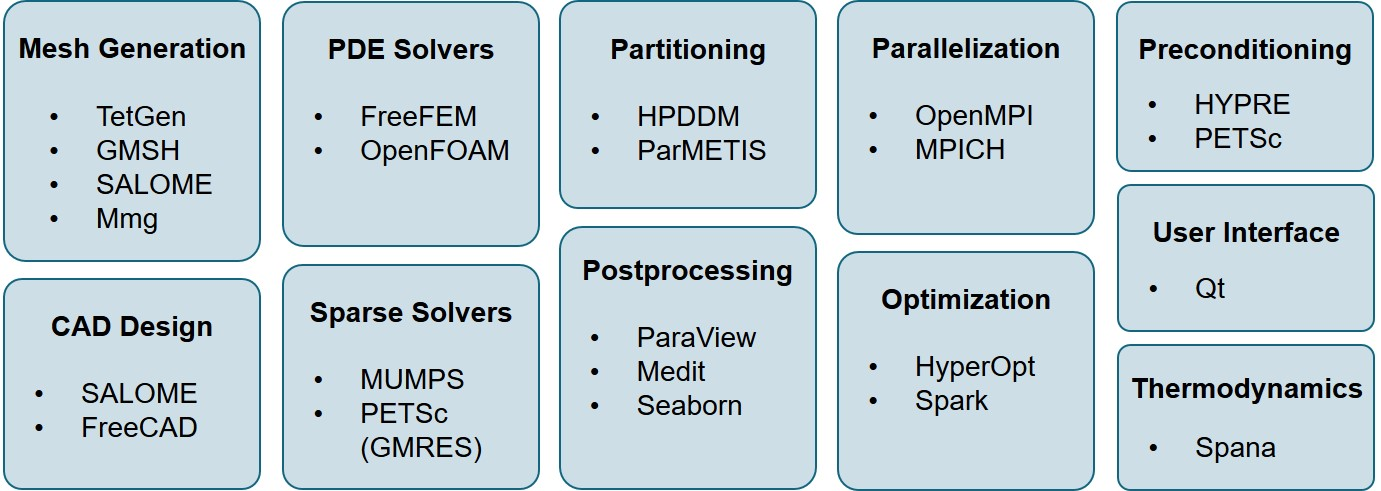
\includegraphics[width=\textwidth]{tools.jpg}
\caption[Overview of open-source tools and libraries used in this PhD]{An overview of tools and libraries used in this research, which are all free and open-source.} \label{fig:conclusion_tools}
\end{figure}

\newglossaryentry{API}{name={API},description={application programming interface}}

One of the most significant advantages of most open-source tools in the scientific computing community is the openness of standards and exchange formats, meaning a custom adapter, application programming interface (\gls{API}), or converter can be developed to import the output of a program into another in case a proper one does not exist. Combined with the flexibility provided by these tools for doing any desired customization, this characteristic makes almost any coupling or exchange possible among various tools. This means that no matter if it is officially supported by the developers, the output of any tool can be used as the input of another. This flexibility was a big advantage for the research performed in this PhD at different levels, for each of which there are many examples to mention from all the chapters. The mesh generation done in Chapter \ref{ch:cup} is a good large-scale example, which was executed using a combination of the FreeFEM internal mesh engine, Mmg, GMSH, and MeshLab on the output of a CGAL-based code. Another relevant example can be the geometry processing and mesh preparation performed in Chapters \ref{ch:core}, \ref{ch:fluid}, and \ref{ch:kinetics}, where an orchestration of various tools, like SALOME, GMSH, meshio, and FreeFEM, made it possible to generate a high-detailed large-scale multi-material mesh for the biodegradation and fluid flow simulations.

The flexibility level provided by open-source tools is not comparable to commercial software programs. This brings two main benefits into play:
\begin{enumerate}
\item
Easier customization to adapt to the target application and usage, which can be observed at various levels. The most-known flexibility in this regard is related to the availability of source codes, making it possible for any researcher to modify the tool to work in the desired manner. Such modifications were useful in some stages of the current PhD, where slight changes were made to some of the interfaces of FreeFEM to behave differently. However, this level is not the only flexibility useful for computational projects. Another prominent possibility is the customization during the build process of the software, meaning that various features of the employed tools can be customized while compiling them from source codes. This is also beneficial from the performance perspective, where building the software from the source codes allows optimizing it to the specific software and hardware configuration of the target system, which leads to increasing the performance and efficiency of the tool. This will be discussed in more details in section \ref{sec:conclusion_hpc}.
\item
More responsive community formed around the tool, providing different levels of help and support for solving users' issues and developing new features. These communities are unique for open-source paradigm as the contributors are not necessarily the main software developers. This relies on the open nature of the software, making it possible for anyone to contribute with different forms of support. This is extremely important and beneficial for more complex tools like the ones typically used in scientific computing and computational science projects.
\end{enumerate}

Another added value of using open-source tools is related to the transparency and reproducibility of the research, a bonus that opens the stage for more efficient science outreach as well. Constructing research using freely available tools means that anyone can re-run the codes and models to reproduce the results, an action that can dramatically increase the transparency of the research and trust in the obtained results. This is still possible in research studies done with proprietary software programs, but the users who want to reproduce the results need to pay for the licenses first. Moreover, the tendency to share the codes, models and workflows is more likely in the open-source community. As mentioned above, this added value has a mutual benefit for both the transparency and science outreach, meaning that sharing the developed models and workflows can be treated as efficient project outreach in addition to increasing trust and transparency. In other words, open-source tools can help project outreach activities meet open science principles. An example of these activities are presented in Chapters \ref{ch:biodeg} and \ref{ch:bayesian}. In Chapter \ref{ch:biodeg}, the developed models are encapsulated into a standalone open-source software that relies on open-source tools to work, implying that the users do not need any additional license to run biodegradation simulations. This software was reviewed and published in the Journal of Open-Source Software (JOSS) \cite{Barzegari2022JOSS}. In Chapter \ref{ch:bayesian}, the details of the utilized parameter estimation process, an important building block of the carried out research, was represented as a self-teaching educational material in the format of Jupyter notebooks. This work was published in the Journal of Open-Source Education (JOSE) \cite{Barzegari2021JOSE}.

A possible advantage of using proprietary codes in the development of medical devices comes with the assistance provided in the regulatory approval process. Digital evidence used in the regulatory dossier requires credibility assessment, following verification, validation and uncertainty quantification (\gls{VVUQ}) guidelines (discussed in section \ref{sec:conclusion_vvuq}).  A big part of the verification is related to the software code itself, and companies owing proprietary codes have often already prepared extensive documentation.  However, as open source codes are maturing, also their developers are developing this sort of verification documentation. An example is FEBio \cite{Maas2012}, a finite element code primarily developed for applications in biomechanics, funded by public money from the NIH in the USA.

As a summary, we should emphasize that this PhD was not possible without the freedom and flexibility available in open-source scientific computing world. The open-source paradigm also helped us to increase the outreach of the project using open science principles. Additionally, it is worth mentioning that in line with the project outreach activities, the obtained knowledge is getting published as a YouTube project called TuxRiders\footnote{\url{https://www.youtube.com/TuxRiders}}, in which the power of open-source scientific computing tools are discussed in details and demonstrated using practical use cases coming from real-world projects, which encompasses the research carried out in this PhD as well.


\subsection{High-performance computing and scaling} \label{sec:conclusion_hpc}

Parallelization of the models has been one of the main objectives of this PhD, making the models run faster to get the predictions and output in less time in large-scale simulations. Achieving this goal has involved various challenges across the project, which can be divided into two main categories: implementation and performance tuning issues. The implementation perspective was discussed in details in Chapters \ref{ch:core}, \ref{ch:fluid}, \ref{ch:hpc}, and \ref{ch:cup}. The main implementation strategy was based on high-performance mesh decomposition, partitioning and distributing the mesh among available computing resources, and then utilization of high-performance preconditioners and iterative solvers tailored for different systems and physics. For example, the FieldSplit preconditioner and blocking approach was used for dealing with the Stokes and Navier-Stokes equations in the fluid flow system, and the BoomerAMG preconditioner was opted for the reaction-diffusion systems after evaluating various available options.

Although it might not appear so, the performance tuning aspect can be as complicated as the implementation \cite{Mikailov2019,Bailey2010}. Running the model using 10 \gls{CPU} cores with an accepted performance and speedup does not mean that one can increase the number of cores to 100 and still get the same speedup. The same problem appears by moving from the order of hundreds to the order of thousands, and so on. Entering a new order of magnitude for the number of \gls{CPU} cores requires dealing with new issues \cite{Hager2011,Goedecker2001,Wadleigh2000}.

This section briefly summarizes various issues one can face while tackling \gls{HPC} and performance-tuning challenges. These experiences were obtained by working in \gls{HPC} environments on the VSC supercomputer in Belgium, the Snellius supercomputer in the Netherlands, and the ARCHER2 supercomputer in the UK. The order in which the items are sorted does not imply their importance. All the mentioned points should be taken into account for optimizing a code to get better performance.

\begin{itemize}
\item
\textbf{Building tools with different \gls{MPI} implementations and toolchains}: Running codes in an \gls{HPC} environment is quite different from a local machine, where all the software and hardware configurations made by the system maintainers can affect the performance of the code. Among various software-related aspects, the chosen compiler toolchain (GNU, Intel, Cray, etc.) and \gls{MPI} implementation (MPICH, OpenMPI, Intel \gls{MPI}, etc.) used to build and run a code can play an important role. In most cases, the computational tools should be built with all the available toolchains and \gls{MPI} implementations to check which one offers better performance on the specific \gls{HPC} environment.
\item
\textbf{Inter-node communication}: Communications taking place between the computing nodes are the source of most of the problems happening in parallelization and performance tuning of codes. The first step towards a faster model is to check the code to remove unnecessary inter-node communications, especially for large-scale simulations. For example, there are usually redundant collective \gls{MPI} calls in the model initialization that can be replaced by encapsulating more work in the main process and performing the collective operations at the end of it. These collective calls usually appear during the first round of parallelization of the code as a result of direct translation from sequential procedures.
\item
\textbf{Running parallel version of tools and codes}: This point is actually a combination of the two previous points from a practical point of view. When a computational tool is built in \gls{HPC} environments, it may fail to run in more than one node due to an inappropriate configuration during the build process. For example, FreeFEM may fail to execute when the job is supposed to run in more than a single node, implying that the inter-node communication does not work due to the used \gls{MPI} or compiler toolchain. This scenario frequently occurs, showing the importance of employing correct toolchains and \gls{MPI} implementations. The proper configuration differs from environment to environment, so the best recommendation would be to check the \gls{HPC} documentation provided by vendors or system maintainers.
\item
\textbf{Mesh generation for large-scale models}: The mesh of the acetabular cup presented in Chapter \ref{ch:cup} had more than 45M tetrahedral elements. Besides the technical aspects of the computational part, generating such a mesh can be quite challenging and time consuming. Some of the common tools used for mesh generation have a parallel version aimed to work with a couple of \gls{CPU} cores to reduce the time needed for mesh generation. For example, Mmg has a parallel version called ParMmg, and CGAL supports shared-memory parallelization for volumetric mesh generation. However, these tools are not very reliable and may cause further problems. In our tests on ParMmg, the tool showed major issues with inter-node communication on large-scale mesh generation, leading us to use sequential mesh generation principles for making the mesh in some cases (Chapter \ref{ch:cup}).
\item
\textbf{Mesh partitioning for large-scale models}: Choosing a proper mesh partitioner plays an essential role in the initialization of the simulations but can also be the source of some failure at this stage. The commonly-used partitioner in this research was METIS software. However, in particular cases and contrary to the previous point for mesh generators, it was observed that its parallel version, called ParMETIS, has significantly better performance. Switching between the sequential and parallel version of this partitioner, as well as using other tools such as SCOTCH, should be considered in the performance tuning of computational models.
\item
\textbf{Memory issues in each node}: Memory-related issues are one of the most common problems one can face while tuning computational models for better scaling behavior. Reviewing code for fixing memory-related issues can reduce memory usage, especially in the initialization stage, helping overcome part of these memory bottlenecks. The memory issues can be debugged in a single node execution first with the maximum memory available. In some cases, one needs to reduce the number of employed \gls{CPU} cores in a node so that more memory is available to each core. Although this action can help remove memory-related errors, it reduces the efficiency of the whole computational task, leaving some \gls{CPU} cores unused in each node due to memory problems.
\item
\textbf{Storage and \gls{IO} bottlenecks}: There are usually different storage volumes available in \gls{HPC} environments, which differ in various aspects such as the speed of access, space limitations, and backup policies. Choosing a proper location for file \gls{IO} can particularly impact the performance of the codes. In more advanced \gls{HPC} environments, the user does not have direct access to high-speed storage, so explicit file operations should be defined in the job batch file describing how the files should be copied to the high-speed volumes and moved back to the home directories. Another storage-related performance bottleneck is the known issue of slowed down reading speed of a large number of small files, which exists in some \gls{HPC} environments. This problem usually impacts remote postprocessing and visualization tasks, in which a large number of files should be processed on an \gls{HPC} node.
\item
\textbf{Remote visualization}: In large-scale simulations, where the model predictions result in tremendous output files, remote postprocessing and visualization can be a more efficient option compared to conventional local processing. Moreover, doing this can be beneficial for the debugging and performance tuning of computational models, where it saves a lot of time needed to transfer the files to a local machine for analysis. For the simulation presented in Chapter \ref{ch:cup}, the results comprise of \num{95000} files with a total size of 148 GB. The visualization was done on a node featuring a \gls{GPU} using the ParaView server on the remote node and the ParaView client on the local machine. Configuring such remote processing requires extra steps in \gls{HPC} environments, such as making secure tunnels and setting up offscreen rendering, which are unnecessary to perform normal computational tasks.
\end{itemize}


\section{Future perspectives}


The research carried out in this PhD can be seen as the first steps for constructing a comprehensive biodegradation model capable of working in 3D for any arbitrary shape and being integrated into other relevant modeling workflows. At its current stage, the model has been calibrated mainly for commercially-pure Mg and has been tested in immersion and hydrodynamics setup for aggressive corrosion environments and buffered solutions. Consequently, different lines of development can be considered to extend the model in the future. These lines can be classified into either developing the core model to improve its methodological aspects or combining it with other models for various use cases and applications.

The future perspective can be seen as an attempt to address the mentioned limitations we faced in various stages and aspects of this research, allowing the developed model to capture more chemical and biological processes and improve its credibility. It is worth mentioning that in addition to improved numerical and computational methodologies, these perspectives require more sophisticated experimental approaches for validation purposes. This aspect of future development is not discussed in this thesis.

\subsection{Other materials and effect of alloying elements} \label{sec:conclusion_alloy}

As stated several times throughout this thesis, biodegradable metals include magnesium, zinc, and iron, among which magnesium is the most studied material. However, zing and iron have been gaining attention in recent years for various applications. As a result, the model can be further developed to capture the biodegradation of iron and zinc as well. Doing this does not need development from scratch since the biodegradation mechanisms of zinc and iron are similar to magnesium, meaning that the underlying reduction-oxidation reactions can be easily converted to the forms of the mathematical model developed in this thesis.

Another factor limiting the applicability of the model developed in this thesis is related to its lack of support for different types of biodegradation other than uniform corrosion. The developed mathematical model, including the reaction-diffusion-convection equations coupled with the level-set formalism for tracking the moving corrosion front, is currently capable of simulating homogeneous corrosion only. Capturing localized corrosion behavior, such as pitting and galvanic corrosion, requires adding the effect of alloying elements and impurities. This needs further development on the core of the mathematical formulation such that it allows the inclusion of active zones in which the rate of degradation is higher.

As part of the work performed in Chapter \ref{ch:infill}, we intended to develop a multi-material biodegradation model capable of simulating the corrosion in composite materials for particular fixation applications in orthopedics. The work lacked a certain theoretical foundation, and as a result, it was not presented in this thesis. However, due to the interesting applications it may have, it should be considered as a worthwhile addition for future developments.

\subsection{Biodegradation in complex electrolytes and environments}

The work presented in Chapters \ref{ch:fluid} and \ref{ch:kinetics} aimed to investigate the biodegradation process in a complex electrolyte in the presence of various contributing chemical components. Doing such modeling combined with the prospective development mentioned in section \ref{sec:conclusion_alloy} would allow the model to mimic the behavior of any metallic biomaterial in any desired environment. However, capturing the biodegradation behavior in complex electrolytes, such as \gls{HBSS} and \gls{SBF}, can be pretty challenging in a mechanistic model, the benefits of which are mentioned in section \ref{sec:conclusion_mechanistic}. In Chapter \ref{ch:kinetics}, the modeling approach was the coupling of the mechanistic model of biodegradation with a thermodynamics-based code being responsible for calculating the concentration of involved chemical species on the corrosion interface. Even though such coupling resulted in acceptable predictions of local pH changes, the extensibility and generalizability of it can still be questionable. A fully mechanistic model, in which the concentration of all components is tracked by means of a set of \gls{PDE}s, can facilitate the model's credibility for such complex environments. This can be considered as an important further development of the model.

Another potential for future research exists in the chemical uncertainty mentioned in section \ref{sec:conclusion_mechanistic}. The uncertainty in various levels of the chemistry of biodegradation, such as the stoichiometry of the precipitation layer in complex electrolytes, is a limiting factor for developing more detailed mathematical models. However, it opens the stage for inverse problem formulations, where the computational model can actually help demystify the complex reactions. As the first step, since the formation of the hydroxyapatite-like precipitation has an unknown stoichiometry (Eq. \ref{eq:kinetics_hydrox_react} in Chapter \ref{ch:kinetics}), an optimization problem can be constructed to find the chemical coefficients such that the simulation output matches the experimentally-obtained values. With such an inverse problem formulation, the computational modeling of the biodegradation process can help experimental research to understand the underlying phenomena better.

\subsection{Uncertainty quantification and model credibility } \label{sec:conclusion_vvuq}

\newglossaryentry{UQ}{name={UQ},description={uncertainty quantification}}

One of the most important limitations of computational models of the biodegradation process is that the majority of them are developed and calibrated for certain systems and under certain conditions. This limitation applies to the model developed in this PhD too. One of the best solutions to tackle this problem is to take advantage of uncertainty quantification (\gls{UQ}) approaches in the context of VVUQ methods. Various methods and techniques provided by UQ can help to assess the model's generalizability, and as a result, enhance its credibility for different biodegradation conditions. UQ may also accelerate the efficient exploration of the effective factors and parameters, resulting in more reliability for the developed model \cite{Albaraghtheh2022}.

UQ is a methodology to characterize the uncertainty in the output of computational models and measure their sensitivity to model parameters, which results in finding the source of uncertainty in the model. An example of a relevant study employing such an approach for building a computational biodegradation model is Zeller-Plumhoff et al. work \cite{Zeller-Plumhoff2022}, in which they used UQ techniques for the parameter estimation of a mechanistic biodegradation model of pure Mg. As demonstrated by this study, employing UQ results in reducing the computational load in the parameter estimation phase and enhancing the generality of the model. Such an analysis should be performed on the model developed in this PhD as further development.

Considering the importance of HPC in this PhD (as discussed in section \ref{sec:conclusion_hpc}), the UQ analysis of the developed biodegradation model should be performed in VVUQ frameworks designed for HPC environments. The suggested framework for this purpose is VECMA\footnote{\url{https://www.vecma-toolkit.eu/}}, an open-source toolkit (www.vecma-toolkit.eu) aimed to provide a wide range of tools to help facilitating the VVUQ processes in developing multiscale and multiphysics computational models, which is developed with scalability in HPC environments in mind \cite{Groen2021}. VECMA has demonstrated it capabilities for a range of different applications - including \textit{in silico} medicine - in recently conducted studies \cite{Suleimenova2021,Suter2021,Vassaux2021,Coveney2021}.


\subsection{Coupled models for a wide range of applications}

As indicated in section \ref{sec:conclusion_summary}, as well as section \ref{sec:aim_objective} in Chapter \ref{ch:objective}, one of the objectives of the research carried out in this thesis was to utilize the developed biodegradation model in various case studies for different applications. Being facilitated by using open-source tools, this objective was demonstrated with three sample studies presented in Chapters \ref{ch:cup}, \ref{ch:infill}, and \ref{ch:mandible}. In these chapters, the biodegradation model was coupled with other mechanical integrity models in order to deliver a more comprehensive representation of the underlying processes in tissue engineering. As an output of these sample use cases, the model showed a big potential from the integration point of view, meaning that it can bring certain added values when being integrated into other modeling workflows.

In addition to the mentioned samples, the model is being used in a few more in-house studies at the time of writing this thesis. One example is the use of the developed model for the evaluation of the biodegradation behavior of different designs of cardiovascular stents in order to move towards an optimal design. Another example is a similar usage of the model to assess and compare the biodegradation rate of various designed screws for orthopedic applications to use the most suitable one for further \textit{in vivo} investigations. In line with all the constructed studies, the developed biodegradation model can be further employed in any other potential modeling use case in tissue engineering and biomaterials science, where biodegradation plays a role that needs to be taken into account. Moreover, further research can be carried out to overcome the challenges mentioned in section \ref{sec:tissue_challenges}, after which the biodegradation model can be coupled with sophisticated tissue growth models to investigate the phenomenon of replacement of biodegradable implants with neotissue happening inside the human body.

By considering the typical applications of biodegradable metallic materials, the impact zone of the developed model will be mostly related to orthopedics and cardiovascular studies. Nevertheless, adding Nerst-Planck terms to the mathematical model enables it to capture the electrochemical potential changes. Doing this allows the model to act as an efficient tool in fundamental research relevant to chemistry and chemical engineering, where the corrosion of metals in aqueous solutions is being studied in the field of electrochemistry. Consequently, it results in a model with a broader application in the field of corrosion science.





%%%%%%%%%%%%%%%%%%%%%%%%%%%%%%%%%%%%%%%%%%%%%%%%%%
% Keep the following \cleardoublepage at the end of this file,
% otherwise \includeonly includes empty pages.
\cleardoublepage

% vim: tw=70 nocindent expandtab foldmethod=marker foldmarker={{{}{,}{}}}
